\section{Event generation}
In order to compare reconstructed data with theoretical predictions, collision events are generated and passed through a simulation of the CMS detector and an emulation it readout. For the detector simulation, a so-called Full Simulation package~\cite{1742-6596-396-2-022003,1742-6596-664-7-072022}  based on the \Geant4 toolkit~\cite{AGOSTINELLI2003250} is employed. It allows a detailed simulation of the interactions of the particles with the detecor material. 
\subsection{Fundamentals of simulating a proton collision}
The procedure of to generate $\Pproton\Pproton \rightarrow \mathrm{X}$ events can be subdivided into sequential steps~\cite{Seymour:2013ega,Sjostrand:2009ad,Hoche:2014rga}, as shown in \fig{fig:ppcollision}.
\begin{figure}[htbp]
	\centering
	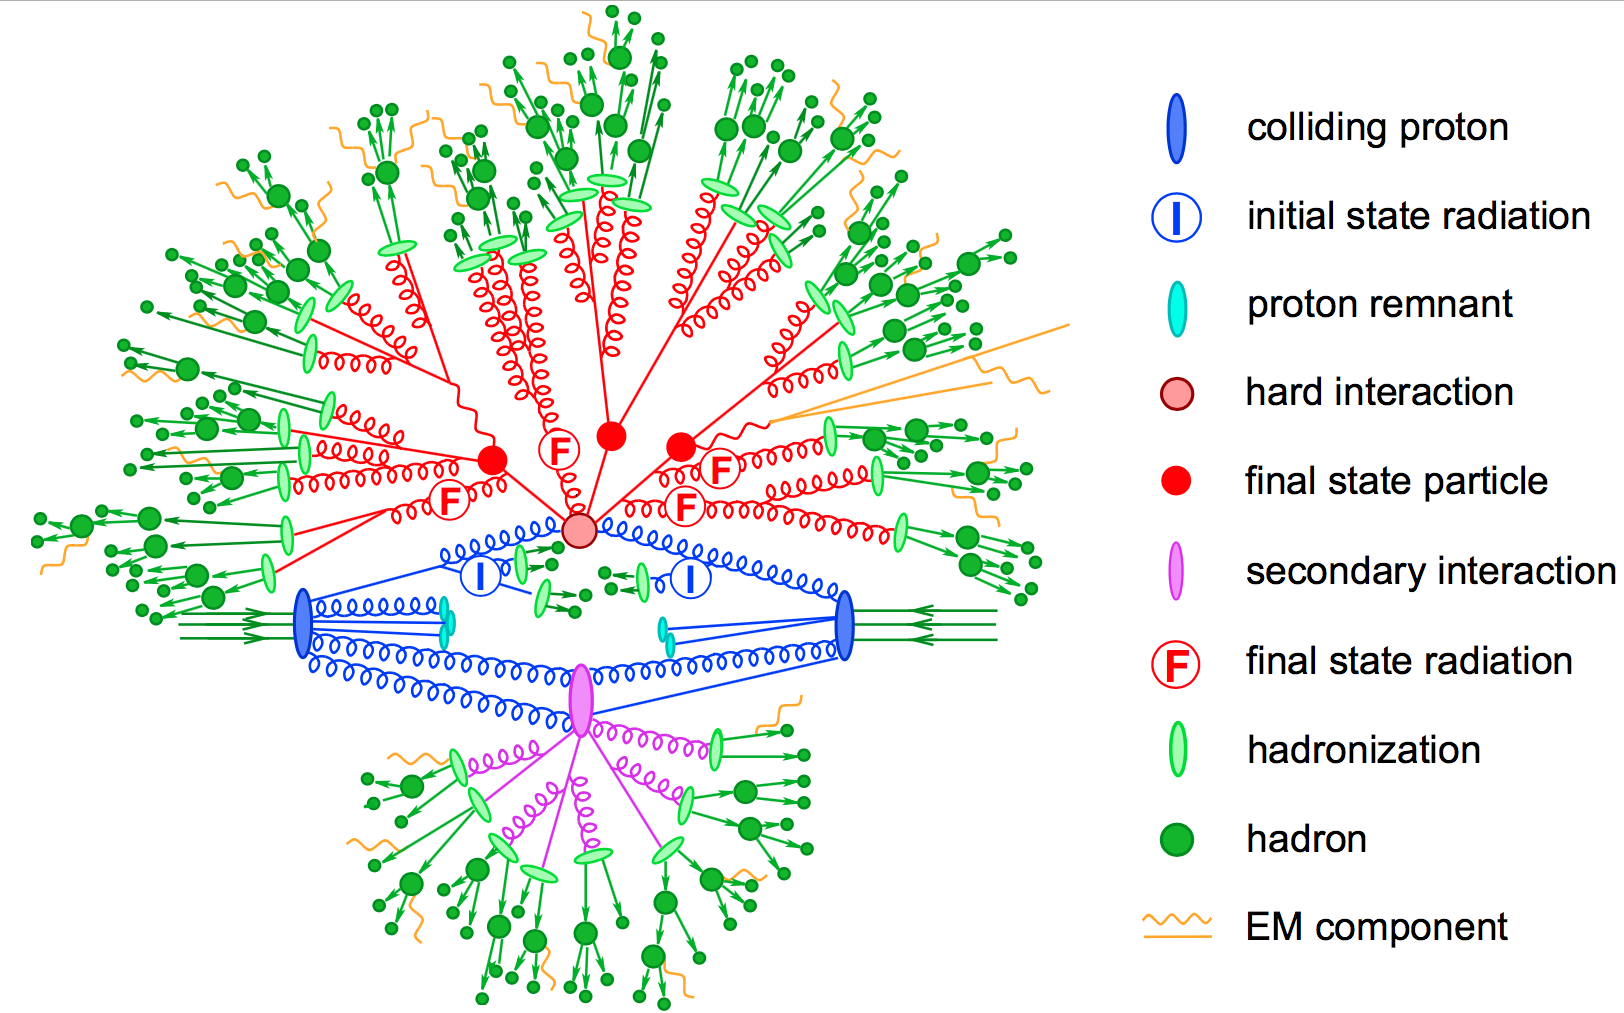
\includegraphics[width=1.\linewidth]{3_Analysis_techniques/Figures/MCeventwithlegend}
	\caption{Sketch of a hadron collision as simulated by a Monte-Carlo event generator. The red blob in the center represents the hard collision, surrounded by a tree-like structure representing Bremsstrahlung as simulated by parton showers. The purple blob indicates a secondary hard scattering event. Parton-to-hadron transitions are represented by light green blobs, dark green blobs indicate hadron decays, while yellow lines signal soft photon radiation. Figure taken from~\cite{Hoche:2014rga}.}
	\label{fig:ppcollision}
\end{figure}

Each proton consists of three valence quarks (\Pup\Pup\Pdown) and many sea quarks and gluons, called partons. These partons emerge from each proton within a certain probability density $f(x,Q^2)$, determined by the momentum fraction $x$ carried by the parton and the momentum transfer $Q^2$. The parton density functions (PDF)~\cite{Placakyte:2011az} give the momentum distribution of the proton amongst its partons.

The interaction of two incoming protons is often soft and elastic leading to events that are not interesting in the framework of this thesis. More interesting are the hard interaction between two partons from the incoming protons. The matrix elements (MEs) of a hard scattering process of interest is the starting point of the generation of events. Monte Carlo techniques are used to sample the corresponding cross section integral and the resulting sample of events reflect the probability distribution of a process over its final state phase space. After obtaining the sample of events of the hard interaction, a parton shower (PS) program is used to simulate the hadronisation of final state partons into hadrons which then can also decay further. Additionally, radiation of soft gluons or quarks from initial or final state partons is simulated. These are respectively reffered to as initial state radiation (ISR) or final state radiation (FSR). Contributions from soft secondary interactions, the so-called underlying event (UE), and colour reconnection effects are also taken into account. \todo{Should I add more details?}
A brief overview of the employed programs used for the event generation of the signal and main background processes used in the search presented in the thesis are given in \Sec{sec:programs}.

\subsection{Programs for event generation}
\label{sec:programs}


%\subsection{Parton distribution functions and the hard interaction}
%\subsection{Parton showering}
%\subsection{Hadronisation and decay}
%explanation of jets https://profmattstrassler.com/articles-and-posts/particle-physics-basics/the-known-apparently-elementary-particles/jets-the-manifestation-of-quarks-and-gluons/
%\subsection{Underlying event}
\begin{comment}
%The draft document may be found at this URL: http://cds.cern.ch/record/2261310
%It is version no. 1 entitled:
%`Measurement of the underlying event using inclusive Z boson production in proton-proton collisions at sqrt(s) = 13 TeV`
% http://cms.cern.ch/iCMS/analysisadmin/cadi?ancode=FSQ-16-008
\end{comment}
%\subsection{Event reconstruction and identification}
% ICHEP https://cds.cern.ch/record/2005743
%\section{Event reconstruction}
\section{Multivariate analysis techniques: Boosted Decision Trees}
\section{Template-based fitting}
%\section{Statistics for a high energy particle physicist}
%\label{sec:Stat}

%\subsection{Boosted decision trees}
%\subsection{Confidence levels }

%https://indico.cern.ch/event/614672/timetable/#20170907
%\subsection{Combine limit setting tool}
%\section{Collision event generation}
